\uuid{gWAF}
\exo7id{5785}
\titre{exo7 5785}
\auteur{rouget}
\organisation{exo7}
\datecreate{2010-10-16}
\isIndication{false}
\isCorrection{true}
\chapitre{Série de Fourier}
\sousChapitre{Calcul de coefficients}
\module{Analyse}
\niveau{L2}
\difficulte{}

\contenu{
\texte{
Développer en série de \textsc{Fourier} la fonction $f~:~x\mapsto x-E(x)-\frac{1}{2}$.
}
\reponse{
La fonction $f$ est $1$-périodique, continue par morceaux sur $\Rr$. On peut donc calculer ses coefficients de \textsc{Fourier}. 

$$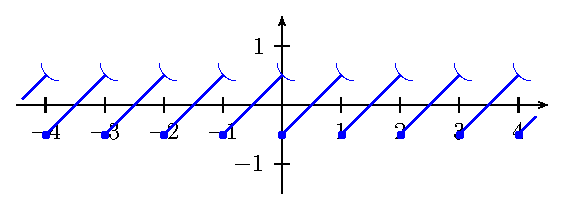
\includegraphics{../images/img005785-1}$$



La fonction $f$ a mêmes coefficients de \textsc{Fourier} que la fonction $g~:~x\mapsto\left\{
\begin{array}{l}
f(x)\;\text{si}\;x\notin\Zz\\
0\;\text{si}\;x\in\Zz
\end{array}
\right.$ qui est impaire. Donc, $\forall n\in\Nn$, $a_n(f)=0$ puis pour $n\in\Nn^*$

\begin{align*}\ensuremath
b_n(f)&=\frac{2}{1}\int_{0}^{1}f(t)\sin\left(\frac{2n\pi t}{1}\right)\;dt=\int_{0}^{1}(2t-1)\sin(2n\pi t)\;dt\\
 &=\left[-\frac{(2t-1)\cos(2n\pi t)}{2n\pi}\right]_0^1+\frac{1}{n\pi}\int_{0}^{1}\cos(2n\pi t)\;dt=\left(-\frac{1}{2n\pi}-\frac{1}{2n\pi}\right)+0\\
 &=-\frac{1}{n\pi}.
\end{align*}

La fonction $f$ est de plus de classe $C^1$ par morceaux sur $\Rr$ et d'après le théorème de \textsc{Dirichlet}, en tout réel $x$, la série de \textsc{Fourier} de $f$ converge et a pour pour somme 
$\frac{1}{2}(f(x^+)+f(x^-))$. En particulier,

\begin{center}
\shadowbox{
$\forall x\in\Rr\setminus\Zz$, $f(x)=x-E(x)-\frac{1}{2}=-\sum_{n=1}^{+\infty}\frac{\sin(2n\pi x)}{n\pi}$. 
}
\end{center}

\item  Soit $p\in\Nn^*$. Pour $n\in\Nn^*$,

\begin{align*}\ensuremath
b_n(f_p)&=2\int_{0}^{1}f(pt)\sin(2n\pi t)\;dt=2\int_{0}^{p}f(u)\sin\left(2n\pi \frac{u}{p}\right)\frac{du}{p}\\
 &=\left[-\frac{(2t-1)\cos(2n\pi t)}{2n\pi}\right]_0^1+\frac{1}{n\pi}\int_{0}^{1}\cos(2n\pi t)\;dt=\left(-\frac{1}{2n\pi}-\frac{1}{2n\pi}\right)+0\\
 &=-\frac{1}{n\pi}.
\end{align*}

\textbf{Remarque.} Soient $p\in\Nn^*$ et $x\in[0,1]\setminus\left\{
\frac{k}{p},\;k\in\llbracket0,p\rrbracket\right\}$. Alors $px\notin\Zz$ et donc

\begin{center}
$f_p(x)=f(px)=-\sum_{n=1}^{+\infty}\frac{\sin(2np\pi x)}{n\pi}=\sum_{k=1}^{+\infty}b_{k,p}\sin(2k\pi x)$
\end{center}

où $\forall k\in\Nn^*$, $b_{k,p}=\left\{
\begin{array}{l}
0\;\text{si}\;k\notin p\Zz\\
-\frac{1}{\frac{k}{p}\pi}\;\text{si}\;k\in p\Zz
\end{array}
\right.$ mais malheureusement, on ne peut pas récupérer ces coefficients car la série obtenue ne converge pas normalement.

\begin{center}
\shadowbox{
$\forall(p,q)\in(\Nn^*)^2$, $\int_{0}^{1}f_q(x)f_q(x)\;dx=\frac{\left(\text{PGCD}(p,q)\right)^2}{12pq}$.
}
\end{center}
}
}
